% Applied Intelligence submission-format draft.
% Official Springer Nature template, numbered sn-basic reference style.
% IMPORTANT: replace the commented author block and declaration placeholders before submission.
\documentclass[pdflatex,sn-basic,Numbered]{sn-jnl}

\usepackage{graphicx}
\usepackage{amsmath,amssymb,amsfonts}
\usepackage[title]{appendix}
\usepackage{booktabs}
\usepackage{microtype}
\usepackage{placeins}
\providecommand{\tightlist}{\setlength{\itemsep}{0pt}\setlength{\parskip}{0pt}}
\raggedbottom
\setlength{\textfloatsep}{8pt plus 2pt minus 2pt}
\setlength{\floatsep}{8pt plus 2pt minus 2pt}
\setlength{\intextsep}{8pt plus 2pt minus 2pt}

\begin{document}

\title[PBIR-GIFT]{Potential-based constraints for LLM-guided reward design in financial reinforcement learning}

% ===== AUTHOR METADATA REQUIRED BEFORE SUBMISSION =====
% \author*[1]{\fnm{Given} \sur{Family}}\email{corresponding.author@example.org}
% \affil*[1]{\orgdiv{Department}, \orgname{Institution},
%   \orgaddress{\city{City}, \postcode{Postal code}, \country{Country}}}

\abstract{Large language model (LLM)-guided reinforcement learning can inject financial knowledge through generated state and reward functions, but adding an unconstrained generated scalar directly to the task reward can distort the investment objective. We propose PBIR-GIFT, a potential-based intrinsic reward extension of the GIFT state--reward interface framework. PBIR-GIFT interprets the generated scalar as a bounded market-state potential and converts changes between consecutive potentials into reward shaping. The existing callable interface is retained, keeping language-model generation offline and requiring no online LLM calls. We evaluate the method on two five-equity subsets derived from the FINSABER benchmark, six rolling half-year windows, and three random seeds using a fixed-code paired protocol. PBIR-GIFT improved mean cell-level Sharpe by 0.278 over Pure GIFT in 10 of 12 dataset--window cells (Hedges' g = 0.940), although the hierarchical-bootstrap 95\% confidence interval {[}-0.010, 0.558{]} marginally crossed zero. The evidence therefore supports a favorable but conditional effect rather than universal superiority, while demonstrating a low-intrusion way to constrain LLM-generated reward interfaces in financial reinforcement learning.}

\keywords{potential-based reward shaping, large language models, financial reinforcement learning, portfolio optimization, reward hacking, generalization}

\maketitle

\hypertarget{introduction}{%
\section{Introduction}\label{introduction}}

\textbf{Background.} Financial portfolio trading requires sequential rebalancing under changing returns, risks, and transaction costs, making deep reinforcement learning (DRL) a natural choice \cite{ref1,ref2,ref3,ref4,ref5,ref6,ref7}. Prior studies improve policy architectures and optimization \cite{ref8,ref9,ref10}, enrich market states with technical, relational, positional, or memory information \cite{ref11,ref12,ref13}, or redesign rewards using smoothing, risk penalties, imitation, and forward-looking objectives \cite{ref12,ref14,ref15,ref16}. More recently, large language models (LLMs) have served as financial agents, signal generators, policy components, and reward designers \cite{ref17,ref18,ref19,ref20}. Together, these methods expand financial RL but leave its state-reward interface insufficiently constrained.

\textbf{Limitations.} Three common limitations motivate this study. \textbf{(1) Accuracy.} OHLCV observations leave relevant financial relationships implicit, while short-horizon returns provide noisy supervision for long-term risk-adjusted performance \cite{ref13,ref14}. \textbf{(2) Efficiency.} Repeated rollouts, multi-agent interaction, and online LLM inference increase training and deployment costs \cite{ref17,ref18,ref19}. \textbf{(3) Generalization.} Hand-designed interfaces may not transfer across assets or regimes, whereas unrestricted LLM rewards may encode spurious patterns, inconsistent reasoning, or weak risk control \cite{ref21,ref22,ref23,ref24}. These limitations call for better reward guidance without another decision layer or LLM inference during portfolio execution.

\textbf{Contributions.} We propose PBIR-GIFT, an environment-side extension of GIFT \cite{ref29}. \textbf{(1) Accuracy.} PBIR reinterprets the LLM-generated scalar as a bounded measure of market-state desirability and rewards improvement between consecutive states instead of adding the scalar directly to the investment reward. \textbf{(2) Efficiency.} Code generation remains offline, the existing callable interface is retained, and portfolio execution requires no online LLM calls. \textbf{(3) Generalization.} The same asset-independent reward transformation is applied across Dataset 1, Dataset 2, and six rolling windows. Mean Sharpe increased by 0.278 in 10 of 12 fixed-code cells, with positive dataset-level differences of +0.220 and +0.336, although the 95\% interval marginally crossed zero. Under its stated assumptions, the transformation preserves the optimal policies of the reference reward, but it does not imply identical finite-sample PPO solutions \cite{ref30}.

\hypertarget{related-work}{%
\section{Related Work}\label{related-work}}

\hypertarget{deep-reinforcement-learning-and-interface-design}{%
\subsection{Deep Reinforcement Learning and Interface Design}\label{deep-reinforcement-learning-and-interface-design}}

Portfolio DRL maps market and holding states to rebalancing actions and learns from return- and risk-related feedback. Research has progressed from direct policy optimization \cite{ref1} to deep multi-asset and relation-aware models \cite{ref2,ref3,ref4}, standard actor--critic algorithms \cite{ref7,ref8,ref9,ref10}, enriched states \cite{ref11,ref12,ref13}, and smoothed, risk-sensitive, imitative, or forward-looking rewards \cite{ref12,ref14,ref15,ref16}.

The common limitation is that most methods optimize the policy while treating the state--reward interface as a fixed design choice. Such interfaces can omit latent financial relations, produce noisy feedback, and require manual redesign when assets or regimes change.

\hypertarget{llm-guided-financial-decision-making}{%
\subsection{LLM-Guided Financial Decision-Making}\label{llm-guided-financial-decision-making}}

Financial LLMs support domain understanding, sentiment analysis, reasoning, and benchmarking \cite{ref25,ref26,ref27,ref28}. Trading systems further use them as agents, signal generators, RL components, and risk-sensitive advisers \cite{ref17,ref18,ref19,ref20}. GIFT instead assigns the LLM an offline role: it generates a state--reward interface while PPO remains the portfolio decision maker \cite{ref29}.

The common limitation is that an unconstrained generated reward can introduce unsupported patterns, inconsistent actions, look-ahead bias, or unstable out-of-sample behaviour \cite{ref23,ref24}. In GIFT, the generated intrinsic reward is still added directly to the trading reward, leaving its influence without a policy-invariant shaping constraint.

\hypertarget{potential-based-reward-shaping}{%
\subsection{Potential-Based Reward Shaping}\label{potential-based-reward-shaping}}

Potential-based reward shaping augments a reference reward with \(F(s_t,s_{t+1})=\gamma\Phi(s_{t+1})-\Phi(s_t)\). Under standard discounted Markov decision-process conditions, this transformation preserves the ordering of optimal policies for the reference objective \cite{ref30}.

Its limitation in the present context is not the shaping theorem itself, but the absence of an established mechanism for constraining an LLM-generated financial reward. PBIR-GIFT connects these lines by treating the generated scalar as \(\Phi(s)\) and letting the environment construct the transition-level shaping term.

\hypertarget{method}{%
\section{Method}\label{method}}

PBIR-GIFT changes only how GIFT's generated scalar enters PPO. The existing portfolio environment constructs states and executes allocations; GIFT generates and validates two callables offline; PBIR interprets the scalar output as a bounded potential and rewards its change between consecutive states. The frozen interface is then reused during PPO training and rolling-window evaluation (Fig.~\ref{fig:method}).

\begin{figure}[!htbp]
\centering
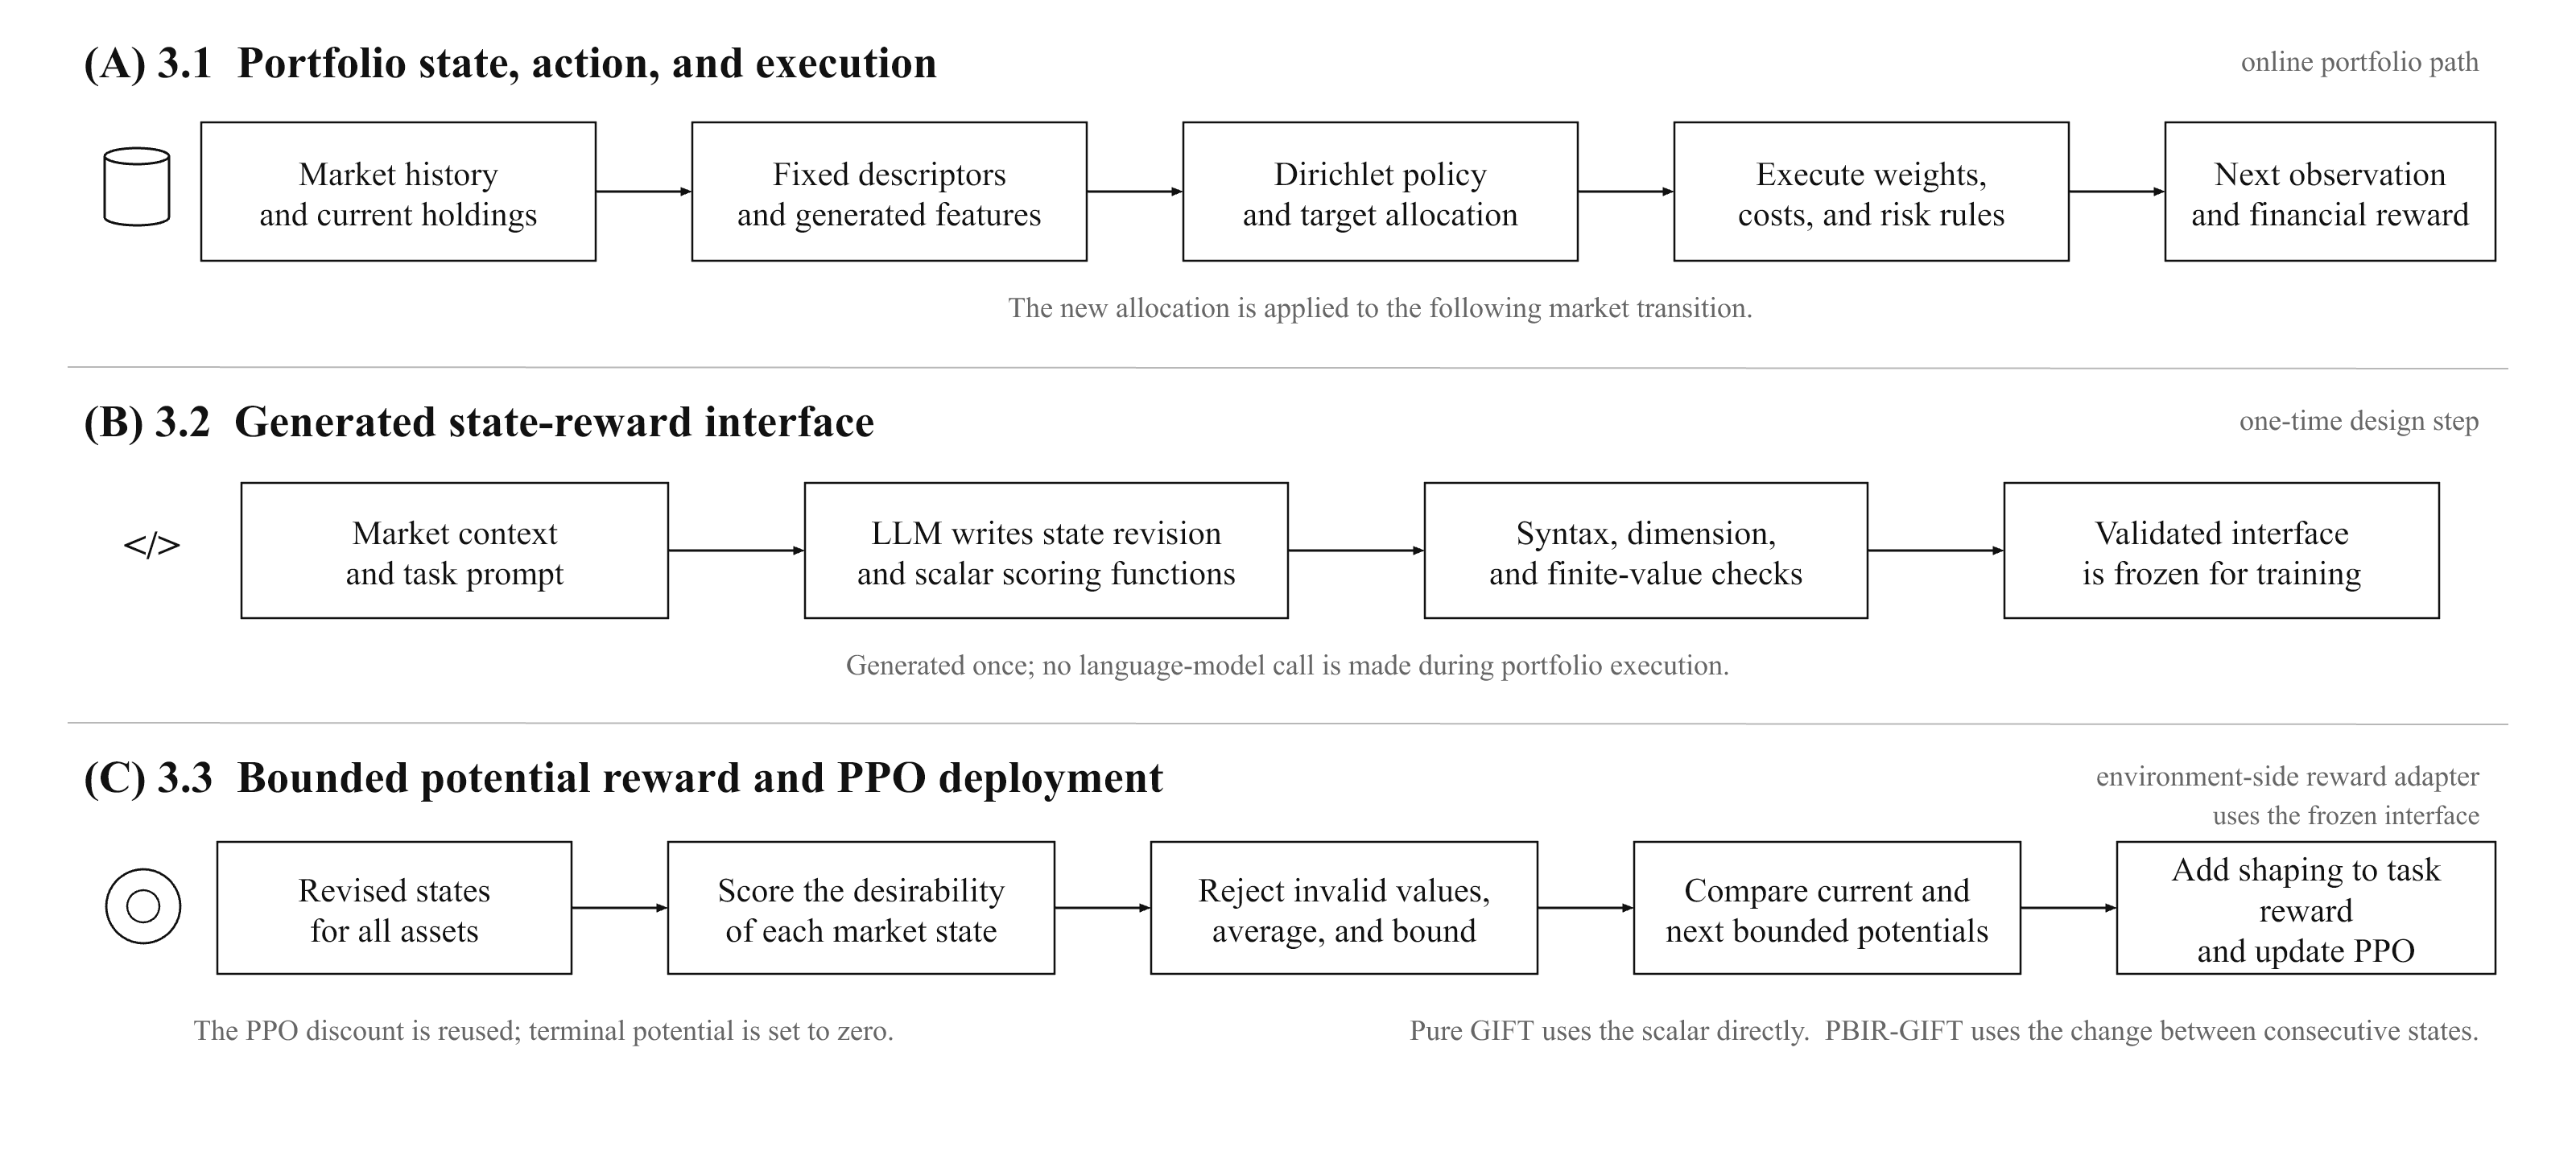
\includegraphics[width=0.94\linewidth]{Fig01.png}
\caption{PBIR-GIFT method. Panels a-c follow Sections 3.1-3.3. Panel a shows portfolio state construction and execution, panel b shows one-time interface generation and validation, and panel c shows bounded potential aggregation, temporal reward adaptation, and PPO deployment.}\label{fig:method}
\end{figure}

\hypertarget{portfolio-state-action-and-execution}{%
\subsection{Portfolio state, action, and execution}\label{portfolio-state-action-and-execution}}

For each of five risky assets, the raw input contains a 20-trading-day history of close, open, high, low, volume, and adjusted close. The environment extracts ten price descriptors per asset: the five most recent closes relative to the 20-day mean and the five most recent close-to-close returns. It then appends finite features produced by \texttt{revise\_state}, a five-dimensional optional portfolio slot, a three-component market-regime vector, and the six current allocations. Missing optional features are filled with zeros. If \texttt{revise\_state} appends K finite features per asset, the policy state has 64 + 5K dimensions; generated features augment rather than replace the fixed representation.

The actor maps this state to positive Dirichlet concentration parameters. Training samples a long-only simplex allocation, whereas evaluation uses the Dirichlet mean. Let \(\mathbf{w}_t\) denote the current weights including cash, \(\mathbf{a}_t\) the target allocation, \(\mathbf{u}_{t+1}\) the next return vector with zero cash return, \(d_t\) the drawdown from the running wealth peak, \(c\) the turnover cost, and \(\lambda\) the drawdown coefficient. The environment credits the price transition to the existing holdings and then applies the new target:

\[
\begin{aligned}
r^{\mathrm{net}}_t&=\mathbf{w}_t^\top\mathbf{u}_{t+1}
-c\frac{\lVert\mathbf{a}_t-\mathbf{w}_t\rVert_1}{2},\\
r_t^{\mathrm{base}}&=r_t^{\mathrm{net}}-\lambda d_t^2,
\qquad \mathbf{w}_{t+1}=\mathbf{a}_t .
\end{aligned}
\]

The action at time \(t\) therefore becomes the holding for the following transition and does not retrospectively earn the current return. The selected \(\lambda\) is frozen with the code artifact. A separate rule term can reward or penalize concentration, diversification, turnover, defensive cash, momentum alignment, volatility scaling, and drawdown behavior.

\hypertarget{generated-statereward-interface}{%
\subsection{Generated state--reward interface}\label{generated-statereward-interface}}

Following GIFT \cite{ref29}, the LLM produces two Python callables. \texttt{revise\_state} must preserve the 120 raw entries and may append finite features; \texttt{intrinsic\_reward} must return a finite scalar. Candidate programs pass abstract-syntax filtering and restricted-namespace checks for function presence, prefix preservation, output dimensions, finiteness, and scalar range. These safeguards validate the expected interface but do not constitute operating-system isolation or prove that arbitrary generated code is safe.

Within each GIFT iteration, a valid interface and its rule configuration remain fixed while a newly initialized PPO agent is trained. Training-return Sharpe selects candidates, and information-coefficient and critic-attribution diagnostics provide textual feedback for later refinements \cite{ref29}. The selected callables, rule parameters, and drawdown coefficient are then frozen. Transfer refers to this interface rather than policy weights: every downstream period trains a fresh PPO agent. Pure GIFT adds the bounded scalar at the next market state directly to the financial and rule rewards.

\hypertarget{bounded-potential-reward-and-ppo-deployment}{%
\subsection{Bounded potential reward and PPO deployment}\label{bounded-potential-reward-and-ppo-deployment}}

PBIR-GIFT retains the name \texttt{intrinsic\_reward} so the sandbox and controller APIs remain unchanged, but changes its mathematical role. For each asset, the function receives the revised 20-day history and returns a state score. The environment keeps finite values, averages them over the valid asset set, and clips the result to the configured bound. It then forms the shaping reward from consecutive potentials:

\[
\begin{aligned}
\Phi(s_t)&=\operatorname{clip}\!\left(
\frac{1}{|\mathcal V_t|}\sum_{i\in\mathcal V_t}\phi_i(s_t),-b,b\right),\\
F_t&=\eta\left[\gamma\Phi(s_{t+1})-\Phi(s_t)\right],\\
r_t^{\mathrm{PBIR}}&=r_t^{\mathrm{base}}+r_t^{\mathrm{rule}}+F_t.
\end{aligned}
\]

If no valid score is available or either callable fails, the potential falls back to zero. Aggregation and clipping prevent one asset from setting the portfolio-level signal directly. The prompt asks for market-state desirability, such as favorable momentum with lower downside risk and volatility, and excludes realized portfolio return. The potential therefore depends on market history and generated market features, not on current allocations, wealth, or the selected action.

The environment reads \(\gamma\) from the PPO configuration and rejects a mismatch. At a terminal transition, the next potential is zero; no nonlinear clipping is applied after the difference. For a fixed bounded deterministic potential, matching discount factors, a fixed initial-state distribution, and zero terminal potential, the discounted shaping sum is

\[
\sum_{t=0}^{T-1}\gamma^tF_t
=\eta\left[-\Phi(s_0)+\gamma^T\Phi(s_T)\right]
=-\eta\Phi(s_0).
\]

This policy-independent constant preserves the optimal policies of the reference financial-plus-rule reward under the stated assumptions \cite{ref30}. It does not preserve the objective induced by Pure GIFT's direct scalar, guarantee identical finite-sample PPO iterates, ensure faster convergence or superior returns, or eliminate reward hacking under function approximation. On a fixed historical price path, differences between the variants reflect the sensitivity of value estimation and policy optimization to reward timing rather than an ability to steer the market into a higher-potential state.

\textbf{Optimization and deployment.} PPO uses a Dirichlet actor and two value critics. Each update follows one complete historical episode. Generalized advantage estimation \cite{ref31} uses the lower critic estimate; advantages are standardized, the actor follows PPO's clipped objective \cite{ref8} with entropy regularization, and the critics use clipped mean-squared error. Generated callables, rule parameters, and the PBIR switch remain fixed within each training call. A later evaluation period reloads the selected interface, trains a fresh PPO policy on its adaptation segment, and uses deterministic mean allocations without online LLM calls. The language model is therefore a design-time component rather than a decision-time trading oracle.

\hypertarget{experiments}{%
\section{Experiments}\label{experiments}}

\hypertarget{experimental-settings}{%
\subsection{Experimental settings}\label{experimental-settings}}

The following subsections define the datasets, comparison protocols, parameter search, and evaluation criteria. All settings were fixed before the final evaluation; no outcome is used to redefine the protocol.

\hypertarget{dataset-source}{%
\subsubsection{Dataset source}\label{dataset-source}}

We use two five-equity datasets derived from the FINSABER S\&P 500 release \cite{ref29}. \textbf{Dataset 1} and \textbf{Dataset 2} each contain 3,524 trading dates from 29 June 2010 to 28 June 2024 and six market channels per equity. Both datasets are evaluated over six rolling half-year windows, each preceded by an adaptation period and a 20-day state warm-up. Windows 1-5 contain 105 evaluated daily returns and Window 6 contains 104. The datasets share three equities and therefore provide complementary robustness evidence rather than independent asset universes.

\hypertarget{comparison-algorithms}{%
\subsubsection{Comparison algorithms}\label{comparison-algorithms}}

We evaluate \textbf{ten comparison methods in three roles}:

\begin{itemize}
\tightlist
\item
  \textbf{Core mechanism control:} Pure GIFT uses the same cached code, rule configuration, artifact hash, and PPO seed as PBIR-GIFT; only the reward transformation changes.
\item
  \textbf{Reinforcement-learning controls:} matched-budget PPO and independently tuned PPO \cite{ref8} test sensitivity to the RL baseline.
\item
  \textbf{External strategy controls:} Equal Weight, SMA, WMA, ATR, Bollinger Bands, Turn-of-the-Month, and XGBoost cover rule-based and supervised alternatives \cite{ref38,ref39,ref40}.
\end{itemize}

The cached comparison estimates the PBIR effect conditional on a selected artifact. External comparisons use recorded full-pipeline GIFT artifacts and are reported separately; no transitive comparison is made across protocols.

\hypertarget{parameter-adjustment}{%
\subsubsection{Parameter adjustment}\label{parameter-adjustment}}

Stage A searches \textbf{five parameter groups in a fixed order} on Dataset 1, Window 1:

\begin{itemize}
\tightlist
\item
  PPO update epochs: 1, 3, 5, 8, and 10;
\item
  maximum training episodes: 20, 35, 50, 75, and 100;
\item
  actor learning rate: 0.00005, 0.0001, 0.0003, 0.0005, and 0.001;
\item
  PPO clipping coefficient: 0.05, 0.10, 0.15, 0.20, and 0.30;
\item
  entropy coefficient: 0, 0.001, 0.005, 0.01, and 0.02.
\end{itemize}

The January-June 2020 interval is divided into adaptation (2 January-31 March) and validation (1 April-30 June). Each step maximizes the mean validation Sharpe across the two methods and freezes earlier selections. The 25 paired selection trials use seed 42; final cached evaluation uses seeds 42, 123, and 456, while PPO is tuned independently with the same three seeds. Because deep-RL results are seed-sensitive \cite{ref32,ref33} and repeated search can inflate backtest performance \cite{ref41,ref42}, these curves are configuration diagnostics rather than causal hyperparameter evidence.

\hypertarget{evaluation-metrics}{%
\subsubsection{Evaluation metrics}\label{evaluation-metrics}}

Evaluation uses \textbf{five performance measures and four inferential checks}:

\begin{itemize}
\tightlist
\item
  \textbf{Primary measure:} annualized Sharpe with a zero risk-free rate \cite{ref34}.
\item
  \textbf{Secondary measures:} Sortino \cite{ref35}, compounded period return, maximum drawdown (MDD), and Calmar. Higher values are preferable except for MDD.
\item
  \textbf{Analysis unit:} one dataset-window cell, averaged over three seeds before paired comparison.
\item
  \textbf{Inference:} positive-cell counts, Hedges' effect size, an exact one-sided sign-flip test, and 10,000 hierarchical circular block-bootstrap resamples \cite{ref36}. Holm correction is applied within each declared comparison family \cite{ref37}.
\item
  \textbf{Strict PBIR criterion:} a positive lower Sharpe confidence bound, positive mean differences in both datasets, at least 8 of 12 positive cells, and no MDD deterioration above five percentage points.
\end{itemize}

\hypertarget{experimental-results}{%
\subsection{Experimental results}\label{experimental-results}}

The main text reports the shortest evidence chain for accuracy, cross-dataset generalization, efficiency, and comparison boundaries. Hyperparameter-selection curves and input-output diagnostics are retained in the Appendix.

\hypertarget{accuracy-and-cross-dataset-generalization}{%
\subsubsection{Accuracy and cross-dataset generalization}\label{accuracy-and-cross-dataset-generalization}}

PBIR-GIFT increased mean cell-level Sharpe by 0.278 over Pure GIFT across 12 fixed-code dataset-window cells. Ten cells were positive (Hedges' \(g=0.940\); one-sided sign-flip \(p=0.0044\); five-metric Holm-adjusted \(p=0.022\)), but the hierarchical-bootstrap 95\% interval {[}-0.010, 0.558{]} crossed zero. The prespecified strict superiority gate therefore failed, supporting a favorable direction rather than universal superiority.

The mean Sharpe difference was positive in Dataset 1 (+0.220; five of six windows) and Dataset 2 (+0.336; five of six), and in odd (+0.368) and even (+0.188) windows. Window-averaged differences ranged from -0.027 in Window 4 to +0.545 in Window 2. This pattern was not confined to one dataset, although shared assets and temporally related windows limit independence.

\begin{figure}[!htbp]
\centering
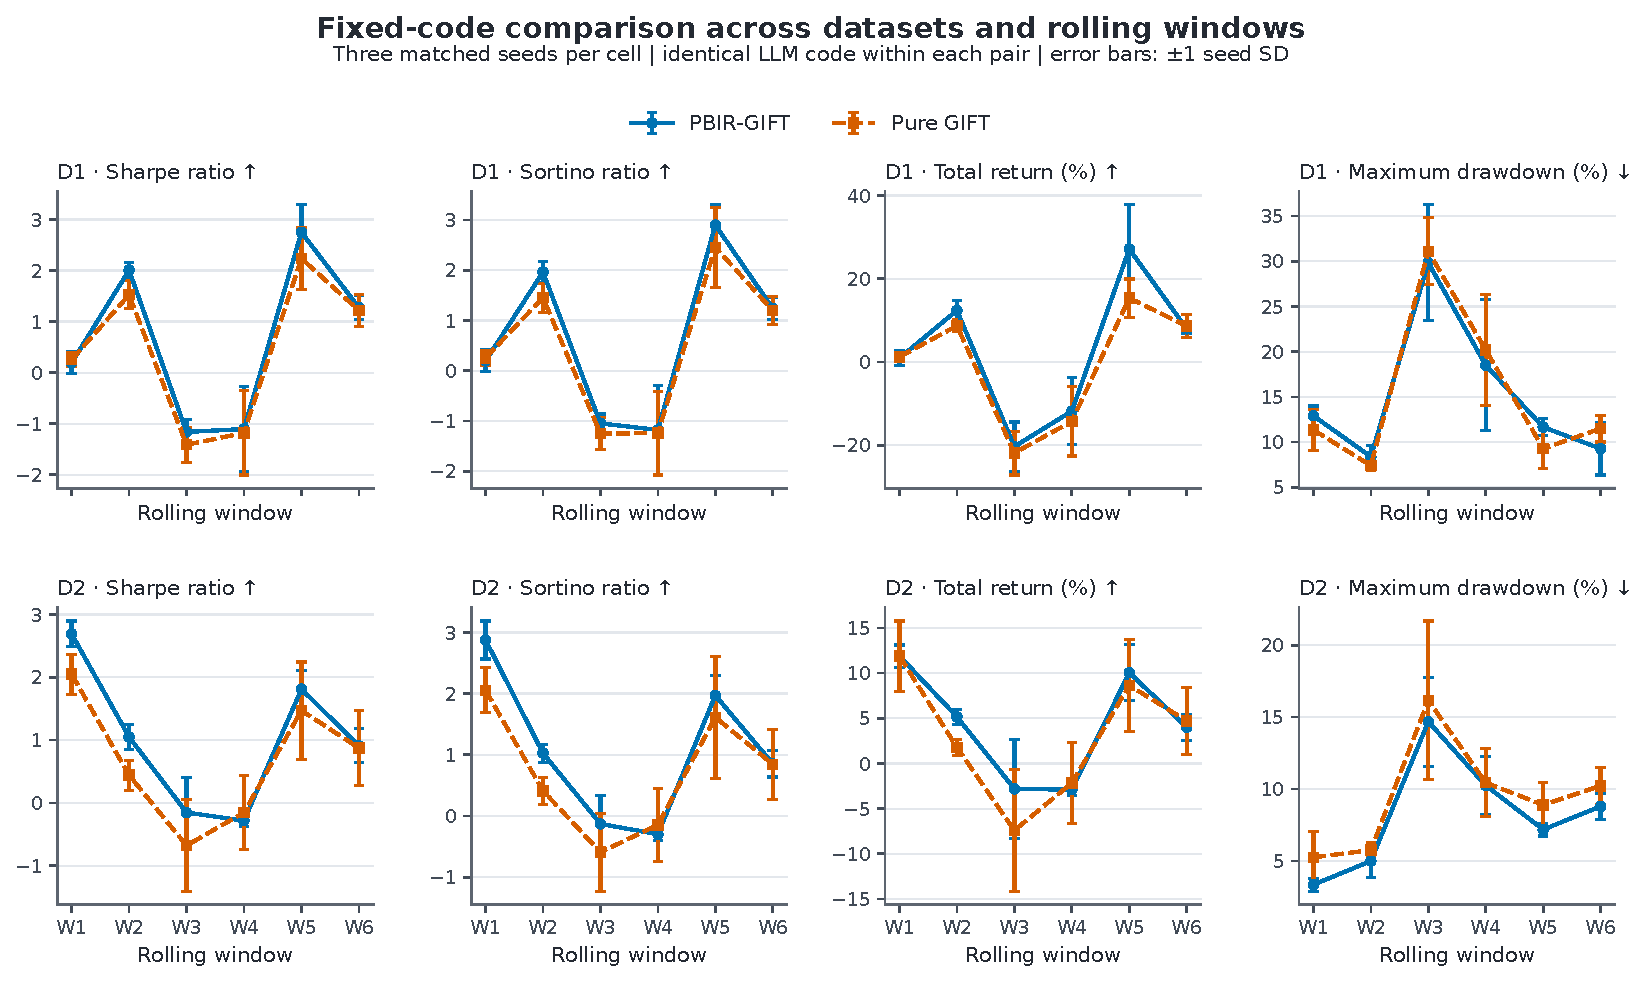
\includegraphics[width=0.88\linewidth]{Fig02.pdf}
\caption{Cross-dataset and cross-window evaluation. Points are three-seed means and whiskers are one sample standard deviation. Returns and MDD are percentages; lower MDD is preferable.}\label{fig:cross-dataset}
\end{figure}

Secondary point estimates were also favorable but uncertain: Sortino +0.276, return +2.205 percentage points, MDD improvement +0.647 points, and Calmar +0.675; every 95\% interval crossed zero. The worst cell-level MDD deterioration was 2.375 points, within the five-point guardrail.

\begin{figure}[!htbp]
\centering
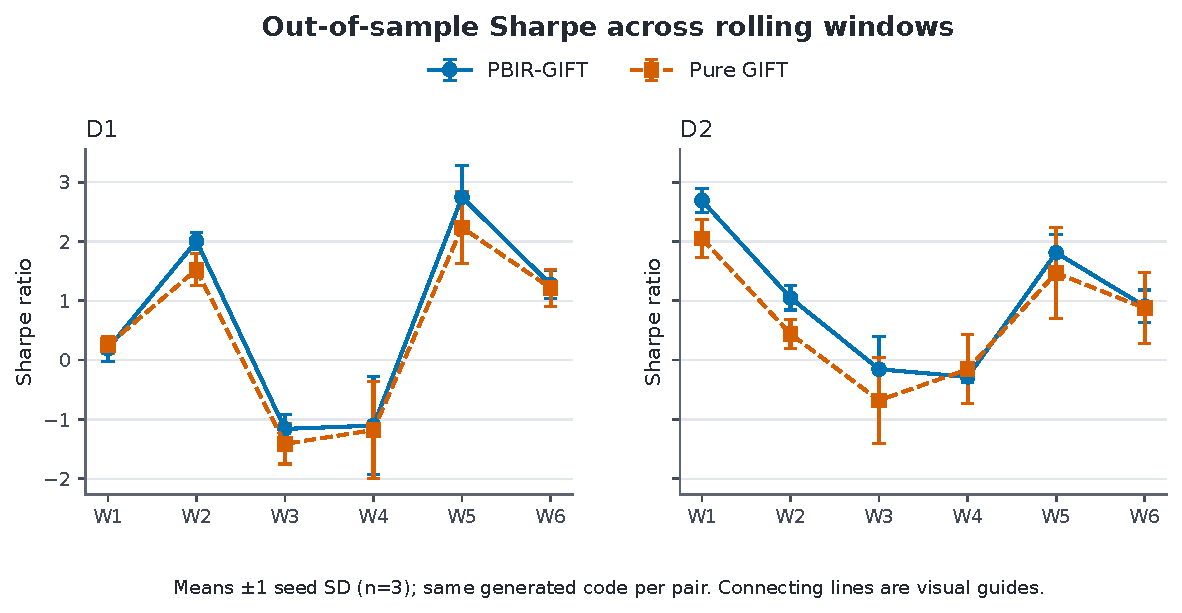
\includegraphics[width=0.82\linewidth]{Fig03.pdf}
\caption{Fixed-code Sharpe by dataset and window. Means plus or minus one seed standard deviation (\(n=3\)); paired methods share identical generated code and differ only in reward transformation.}\label{fig:fixed-code}
\end{figure}

\FloatBarrier
\hypertarget{efficiency-and-baseline-boundary}{%
\subsubsection{Efficiency and baseline boundary}\label{efficiency-and-baseline-boundary}}

All 72 cached method runs made zero LLM calls, isolating downstream training from repeated code generation. The median PBIR-to-Pure runtime ratio was 1.008 across 36 pairs, but unstandardized hardware load and one 9.30-hour outlier preclude speed or runtime-equivalence claims (Fig.~\ref{fig:runtime}).

\begin{figure}[!htbp]
\centering
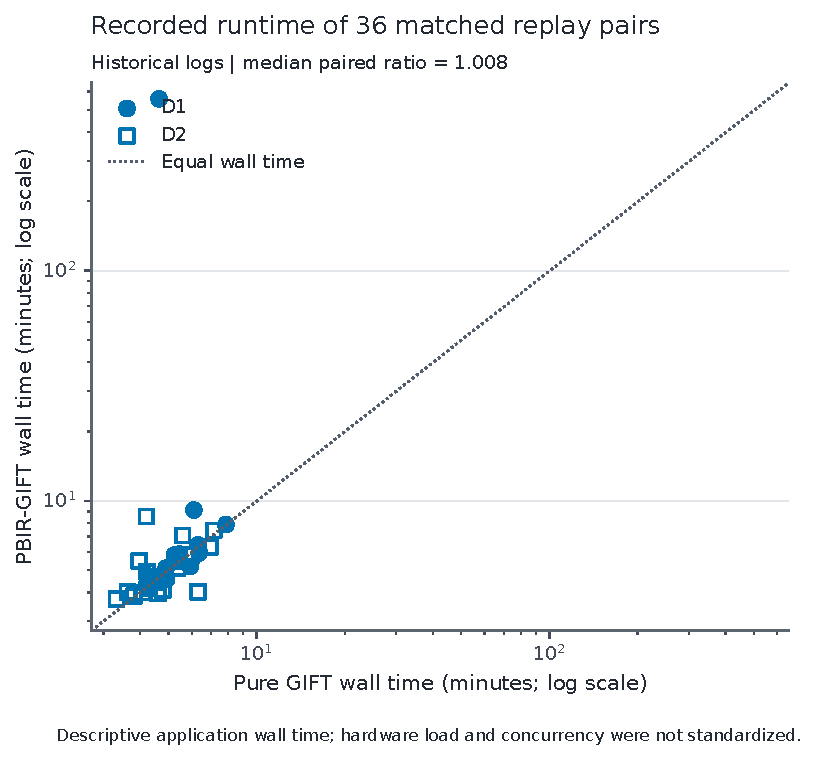
\includegraphics[width=0.68\linewidth]{Fig04.pdf}
\caption{Recorded application runtimes. Each point is one matched dataset-window-seed pair; the diagonal denotes equal runtime. Timings are descriptive, not a controlled GPU benchmark.}\label{fig:runtime}
\end{figure}

Baseline comparisons further bound the claim (Fig.~\ref{fig:contrasts}). Pure GIFT differed from matched PPO by +0.112 and from independently tuned PPO by -0.144; neither interval excluded zero. Its positive contrasts with SMA, Bollinger Bands, and XGBoost also failed the joint multiplicity-and-interval gate. Thus, the strongest evidence remains the conditional PBIR-versus-Pure GIFT comparison under shared code, not general GIFT superiority over strong PPO.

\begin{figure}[!htbp]
\centering
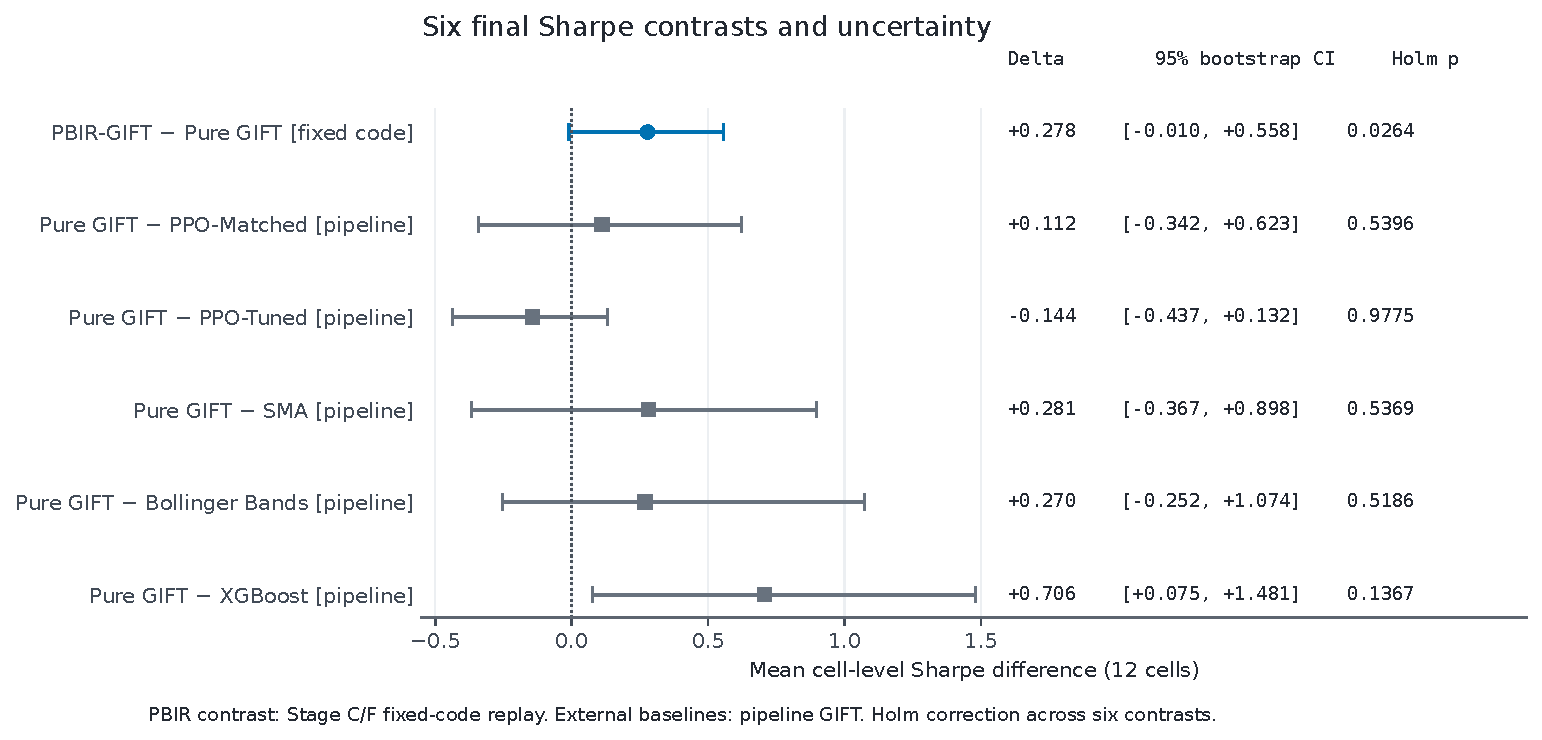
\includegraphics[width=0.86\linewidth]{Fig05.pdf}
\caption{Six final Sharpe contrasts. Horizontal intervals are 95\% hierarchical block-bootstrap intervals; the right column reports Holm-adjusted one-sided sign-flip values. The PBIR row uses fixed-code results, whereas external baselines use their recorded full-pipeline sources, so rows are not transitive comparisons.}\label{fig:contrasts}
\end{figure}

\FloatBarrier
\hypertarget{conclusion}{%
\section{Conclusion}\label{conclusion}}

PBIR-GIFT reinterprets GIFT's generated scalar as a bounded market-state potential and applies an environment-side temporal-difference reward while retaining the original callable interface. Across two datasets and six windows, Sharpe improved by 0.278 in 10 of 12 fixed-code cells, although the 95\% interval marginally crossed zero and strong PPO superiority was not established. Future work should tune potential scale and portfolio-aware potentials on preregistered, non-overlapping markets while benchmarking runtime and transaction-cost sensitivity under standardized hardware.

\clearpage
\begin{appendices}

\hypertarget{hyperparameter-selection}{%
\section{Hyperparameter selection}
\renewcommand{\thefigure}{\arabic{figure}}
\setcounter{figure}{5}\label{hyperparameter-selection}}

\hypertarget{sequential-selection-results}{%
\subsection{Sequential selection results}\label{sequential-selection-results}}

Stage A selected 10 PPO update epochs, 50 training episodes, an actor learning rate of 0.0005, a PPO clipping coefficient of 0.30, and an entropy coefficient of 0.001. Each level was run once with seed 42 and independently generated code, so the plots document configuration selection rather than causal hyperparameter effects or uncertainty intervals.

\begin{figure}[!htbp]
\centering
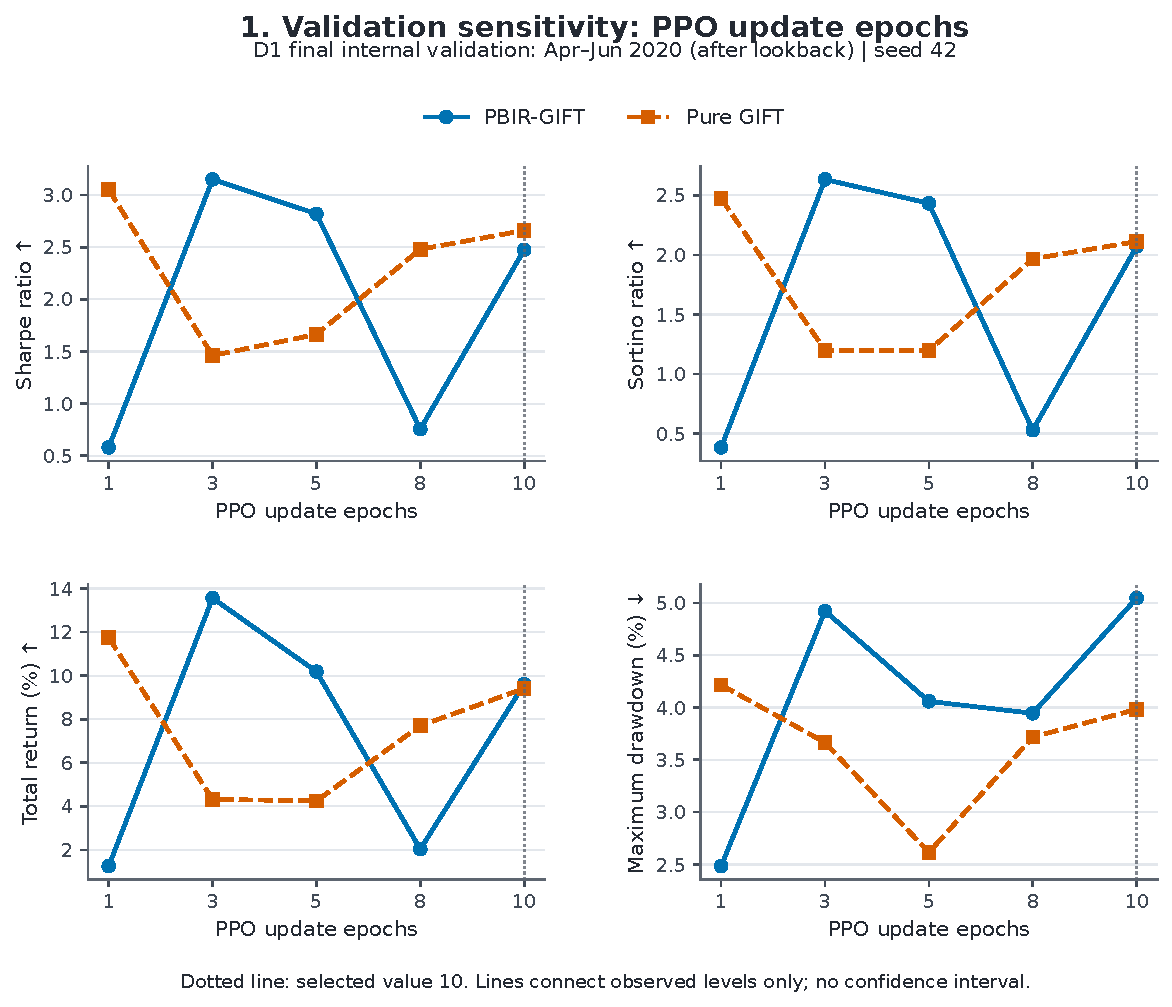
\includegraphics[width=0.92\linewidth]{Fig06.pdf}
\caption{Update-epoch sensitivity. Internal-validation metrics for PBIR-GIFT and Pure GIFT; the dotted line marks the joint selection.}\label{fig:epochs}
\end{figure}

\begin{figure}[!htbp]
\centering
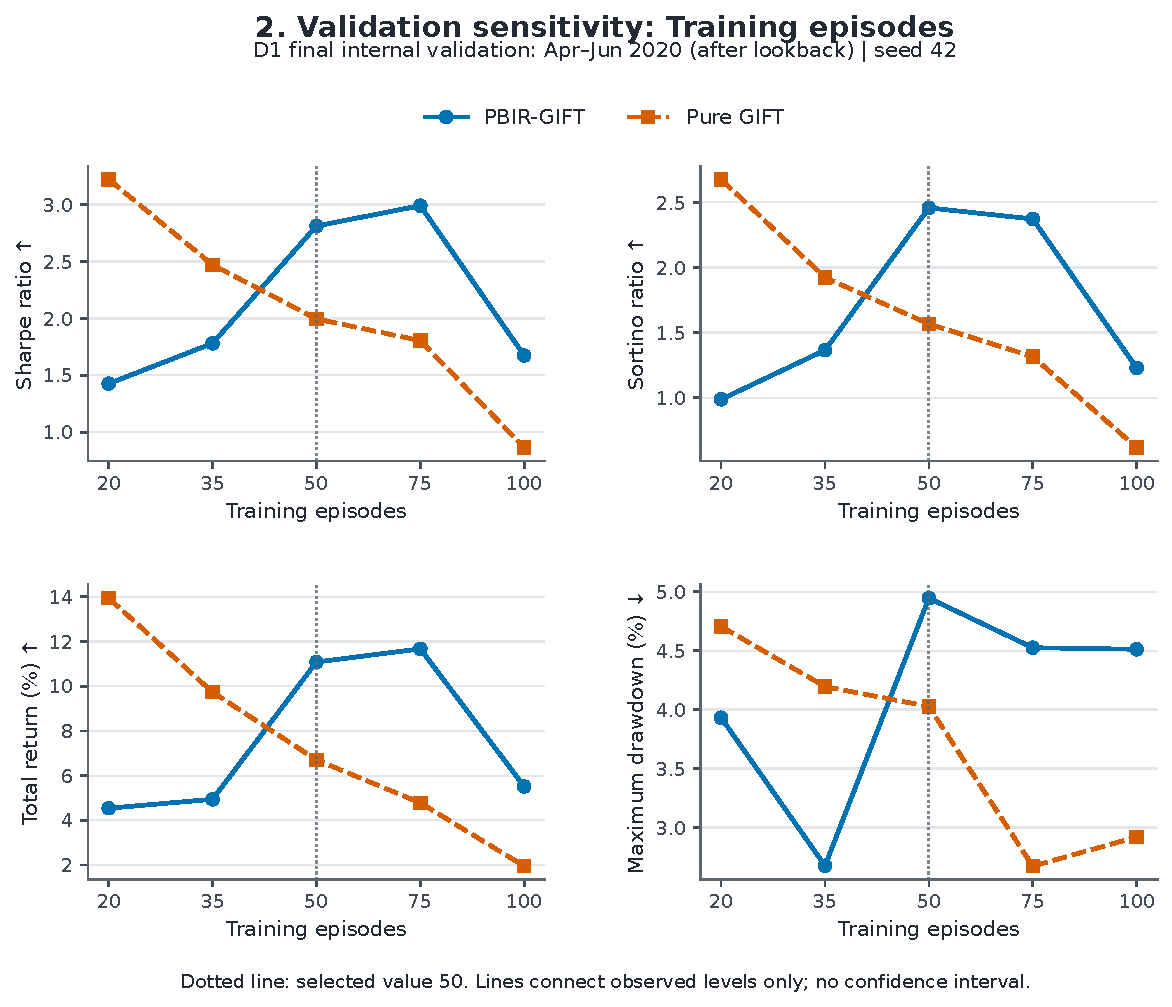
\includegraphics[width=0.92\linewidth]{Fig07.pdf}
\caption{Training-episode sensitivity. Internal-validation metrics after freezing the epoch choice; the dotted line marks the joint selection.}\label{fig:episodes}
\end{figure}

\begin{figure}[!htbp]
\centering
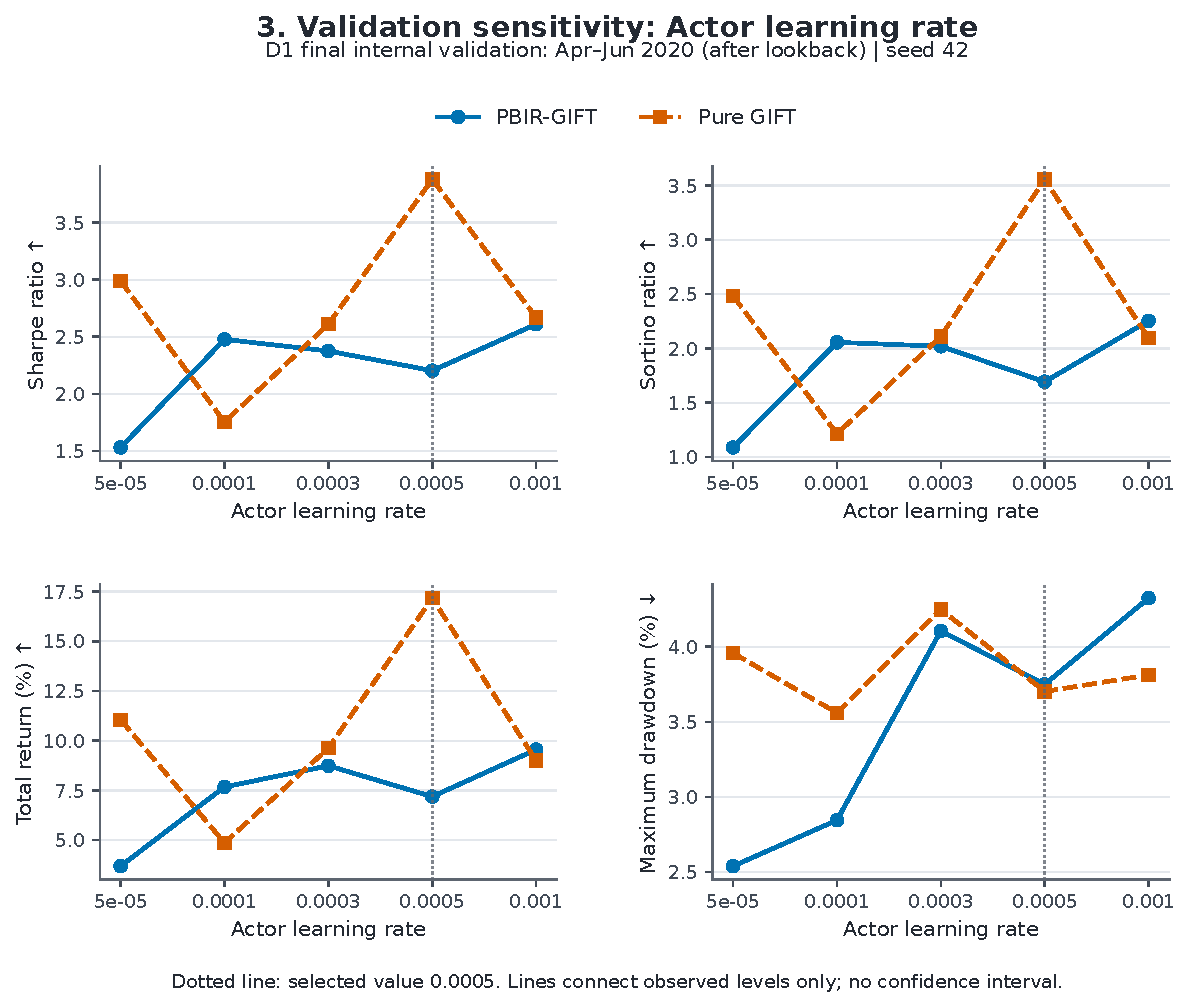
\includegraphics[width=0.92\linewidth]{Fig08.pdf}
\caption{Actor-learning-rate sensitivity. Internal-validation metrics after freezing prior selections; the dotted line marks the selected rate.}\label{fig:learning-rate}
\end{figure}

\begin{figure}[!htbp]
\centering
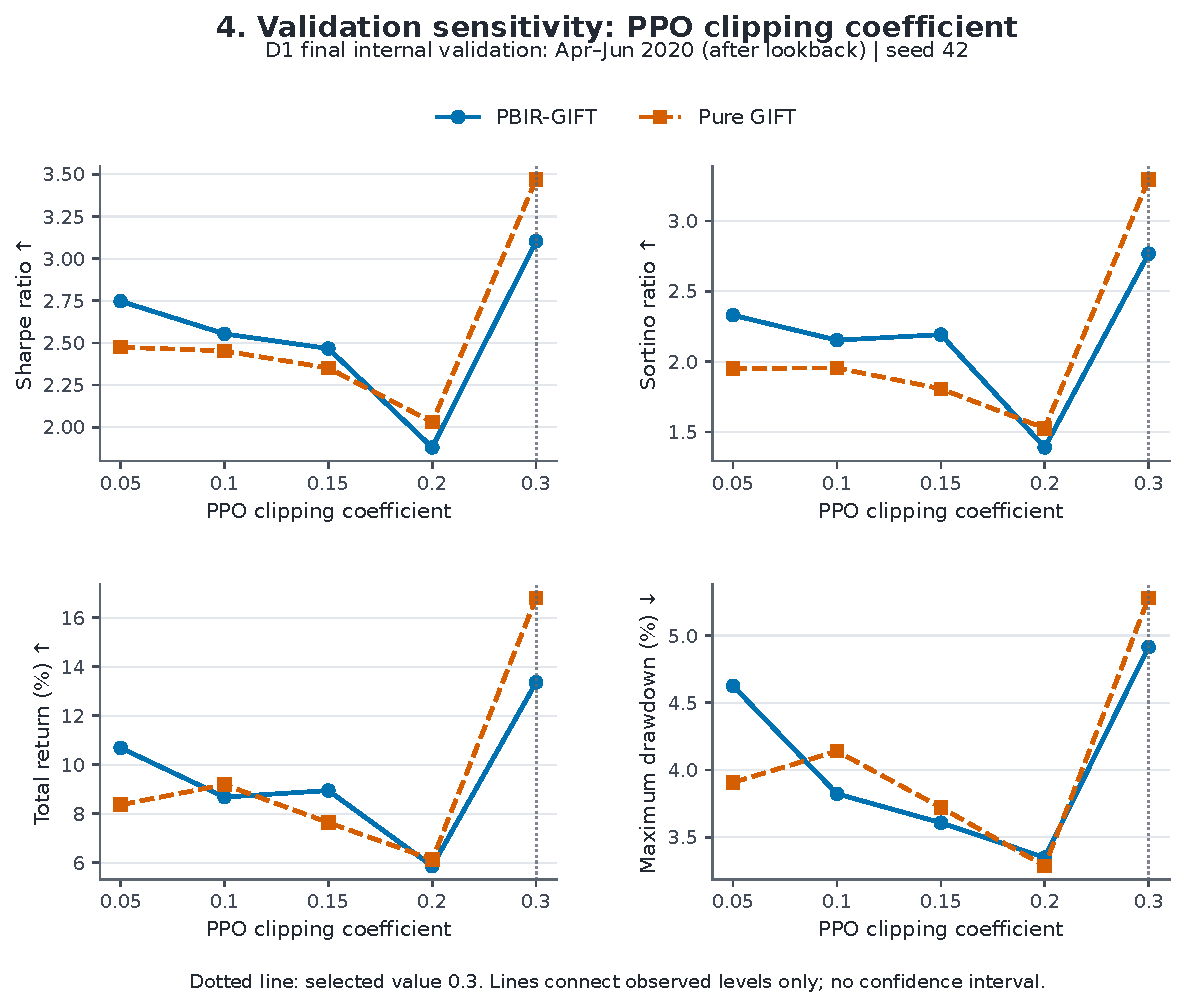
\includegraphics[width=0.92\linewidth]{Fig09.pdf}
\caption{PPO-clipping sensitivity. The selected coefficient lies at the search boundary and is therefore the best observed level, not an unconstrained optimum.}\label{fig:clip}
\end{figure}

\begin{figure}[!htbp]
\centering
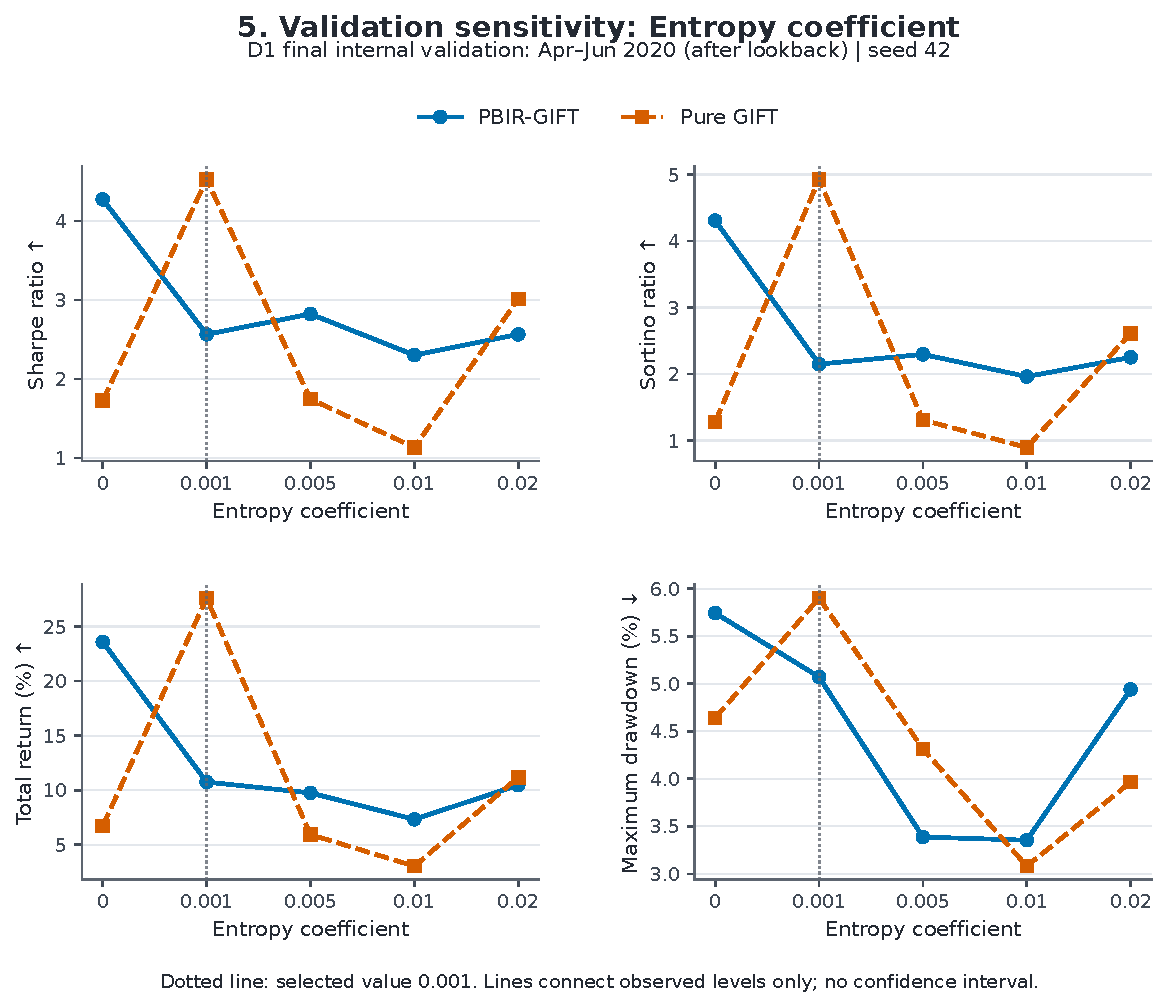
\includegraphics[width=0.92\linewidth]{Fig10.pdf}
\caption{Entropy-coefficient sensitivity. Internal-validation metrics after freezing the first four parameter groups; the dotted line marks the joint selection.}\label{fig:entropy}
\end{figure}

\hypertarget{input-and-output-diagnostics}{%
\FloatBarrier
\section{Input and output diagnostics}
\renewcommand{\thefigure}{\arabic{figure}}
\setcounter{figure}{10}\label{input-and-output-diagnostics}}

The diagnostic figures report all input trajectories, wealth paths, and average allocations rather than selected successful cases. They support traceability and behavioral inspection but do not identify a causal allocation mechanism.

\begin{figure}[!htbp]
\centering
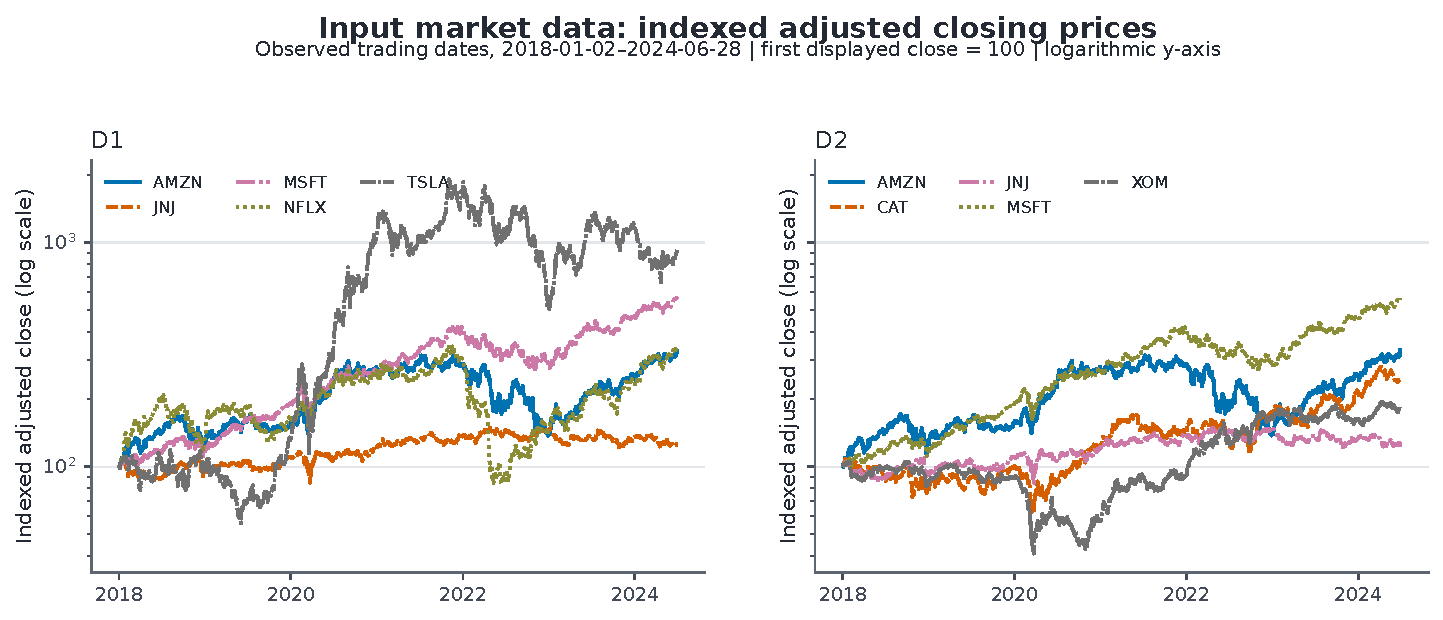
\includegraphics[width=0.99\linewidth]{Fig11.pdf}
\caption{Input data in Dataset 1 and Dataset 2. Adjusted closes are normalized to 100 on 2 January 2018 and shown on a log scale. No values are imputed, and normalization is not the model's preprocessing transform.}\label{fig:inputs}
\end{figure}

\begin{figure}[!htbp]
\centering
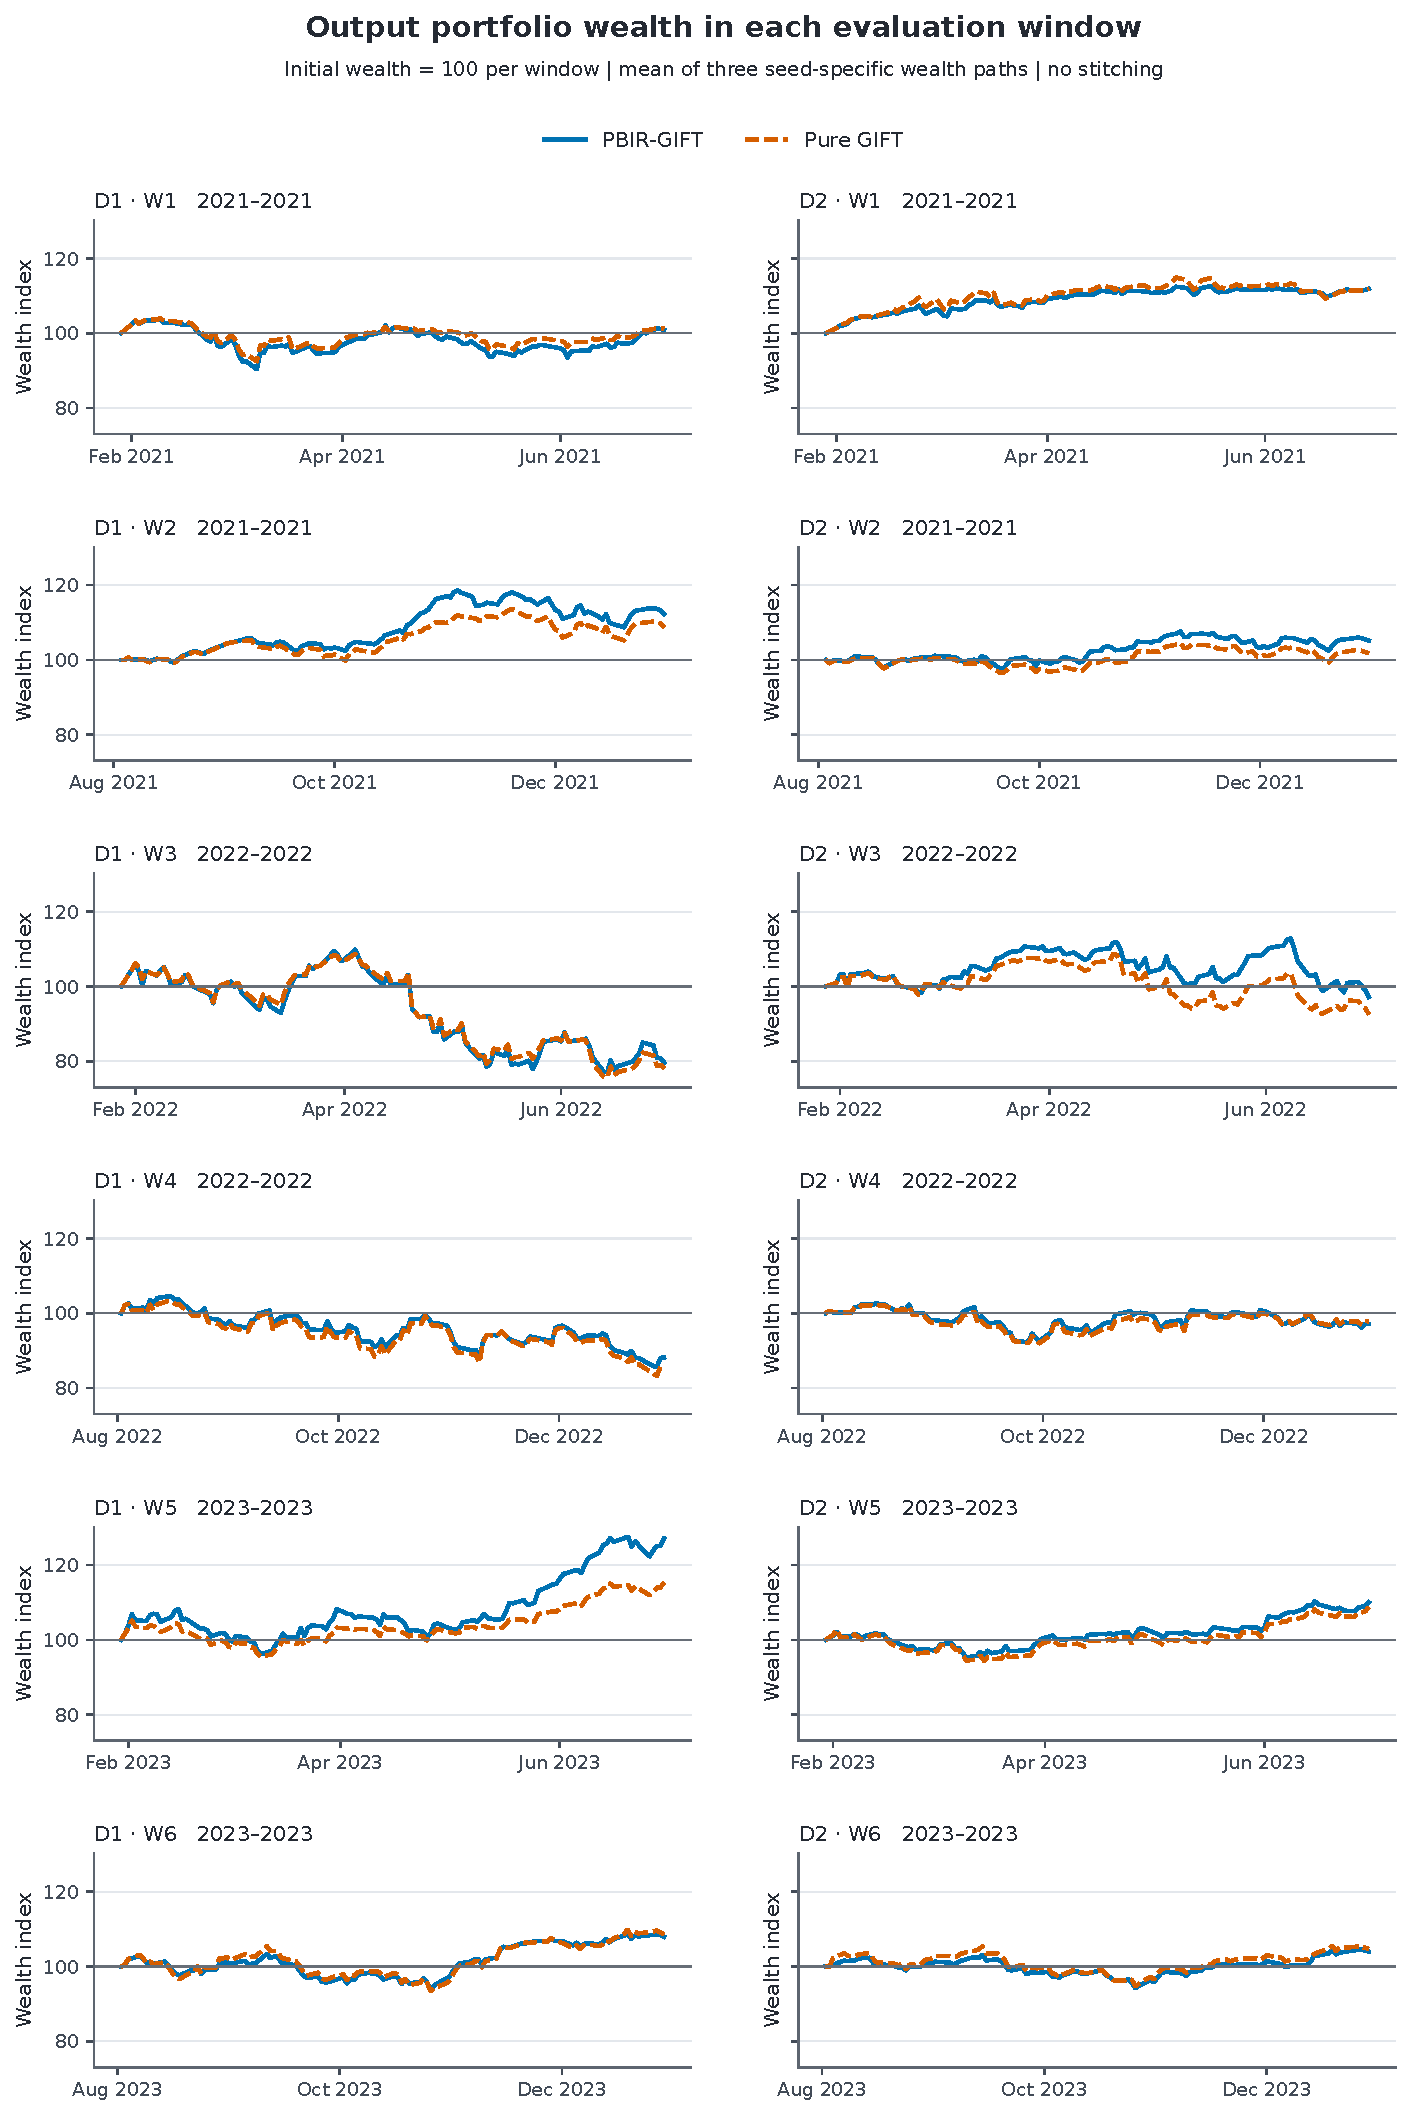
\includegraphics[width=0.90\linewidth]{Fig12.pdf}
\caption{Output wealth paths for all 12 dataset-window cells. Each path starts at 100 and averages three seed-specific wealth indices. Windows restart independently; no smoothing or confidence ribbon is applied.}\label{fig:wealth}
\end{figure}

\begin{figure}[!htbp]
\centering
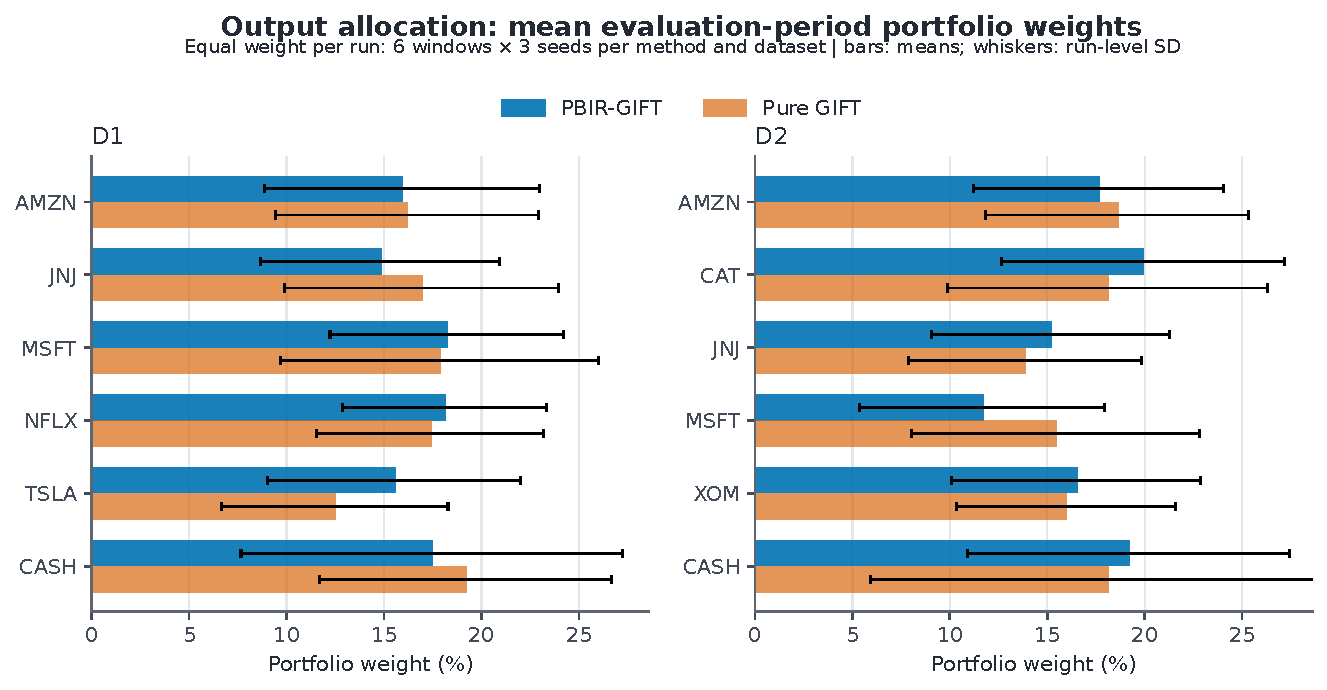
\includegraphics[width=0.92\linewidth]{Fig13.pdf}
\caption{Evaluation-period allocation outputs. Bars average all 18 window-seed run weights per method and dataset, including cash; whiskers are descriptive standard deviations, not confidence intervals.}\label{fig:weights}
\end{figure}
\FloatBarrier
\end{appendices}

\section*{Declarations}

\textbf{Funding} \emph{Author input required before submission.}

\textbf{Competing interests} \emph{Author input required before submission.}

\textbf{Author contributions} \emph{Author names and contribution roles are required before submission.}

\textbf{Data availability} The experiments use two processed five-equity subsets derived from the FINSABER benchmark cited in this article. The public repository will provide preprocessing instructions and integrity checks; redistribution of processed market data remains subject to the source dataset's terms.

\textbf{Code availability} The implementation, experiment manifests, and reproducibility instructions are prepared for release in the accompanying GitHub repository. The final public URL and archived release identifier must be inserted before submission.

\textbf{Ethics approval and consent to participate} Not applicable.

\textbf{Consent for publication} Not applicable.

\bibliography{references}

\end{document}
